\documentclass{standalone}
% preamble: usepackage, etc.
\begin{document}

\chapter{强化学习基础}

强化学习是一种学习如何进行控制和决策的框架,强化学习的灵感来自于仿生学,它完成了从当前的环境状况到行为的映射,并通过学习这一映射过程使得从环境中得到的奖赏值最大化。这样一种框架被誉为可能是发展为强人工智能的框架,包括博弈论、控制理论、群体智能、多智能体系统等领域都与强化学习可以进行结合和交叉。在控制领域,强化学习被视为一种拟合动态规划方法。在博弈论领域,它被用来解释均衡点的出现及其原因。它和有监督学习,无监督学习组成了机器学习领域三个基本的学习框架。它不同于有监督学习和无监督学习,原因在于,在强化学习中,并不存在类似于有监督学习中的标签信息,只有奖赏信号用于指导整个学习过程,同样这也不同于无监督学习中没有任何信号和标签指导学习过程。\par

\section{智能体建模方法和马尔科夫决策过程}
\subsection{智能体建模方法}
强化学习框架的设计一般基于智能体建模的方式实现,基于智能体的模型是一种为了模拟控制和交互的计算模型,这样一种框架包括智能体和环境两类主体,其在多个领域都有广泛的应用,如在生物学中用于研究种群的分布,人口变化等问题,在经济和社会学中,用于研究城市人口流动和城市规划问题,消费者行为分析等。在强化学习中,我们通过图4-1所示的框架对强化学习进行建模。Agent 表示智能体,即表示我们的控制算法的主体。Environment 表示环境,智能体与环境进行交互。在路径规划问题中,智能体代表了我们的路径规划算法,它输出控制车辆的行为如直行,左转等,而环境代表了实际的地图环境,如我们在第2章节所述的多个场景等。
\begin{figure}[h]
	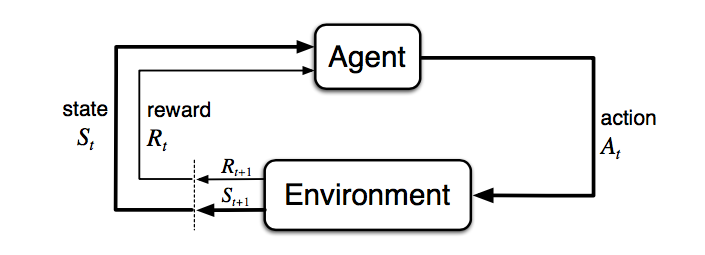
\includegraphics[width=12.0cm]{pic/4-1.png}
	\caption{强化学习框架}
	\label{4-1}
\end{figure}
\subsection{马尔科夫决策过程}
马尔科夫决策过程(Markov Decision Process, MPD)为建模决策问题提供了一个数学框架,MPD对于通过动态规划或强化学习解决和研究优化问题十分重要。这一框架最早于1950年提出,随后 Ronald A. Howard 在书中做了详细做了详细的研究。
在强化学习中,我们通常把环境规范到马尔科夫决策过程,这样的设计有利于强化学习算法的设计,同时便于算法的相关理论证明。\par
精确的来说,智能体和环境在一个离散的时间序列$t=0,1,2,3,... ..$上进行交互,在一个时刻$t$上,智能体接受到表示环境状态的信息(state),随后根据自己身的策略和决策系统,给出行为(action)。环境在接收到该行为后,依据某一概率转移矩阵,进行状态的更新,同时计算一个对应的奖赏信号(Reward),环境把新的状态和奖赏信号返回给智能体,此时进入下一个时刻,该过程不断重复直到环境返回一个结束信号。因此根据以上描述,我们定义一个马尔科夫决策过程是一个包含5个元素的元组,表示为$MDP=(S, A, P_{a}, R_{a}, \gamma)$,其中$S$为一个表示状态的有限集合。$A$表示一个行为的有限集合,更特别的用$A_s$表示某一状态$s$下的可取的行为的集合。$P_a(s, s') = \mathbb{P}(s_{t+1} = s'|s_t = s, a_t=a)$表示在$t$时刻,状态为$s$,采用行为$a$时,$s_{t+1}$为$s'$的概率。$R_a{s, s'}$表示在$t$时刻,状态为$s$,采用行为$a$,状态转移到$s'$时,环境的即时奖赏值。$\gamma \in [0, 1]$表示折扣因子,表示我们主观对即时奖赏和未来奖赏重要程度的差别。\par 

\section{强化学习}
强化学习的目标在于找到一个策略(Policy)使得在该策略下,智能体能够最大化其从环境中受到的累计奖赏值。因此在控制或者决策问题中,我们假设我们的目标或目的即为最大化累计奖赏,这一假设成为奖赏假设。而这一形式也是强化学习相比于其他机器学习框架独特所在。\par
策略定义为:$\pi(a|s) = \mathbb{P}[a_t=a | s_t=t]$,即策略为一个给定状态的行为的概率分布。策略完全定义了一个智能体的行为,同时其决策只依赖于当前时刻的状态。
因此在一个决策过程中,给定$MDP=(S, A, P_{a}, R_{a}, \gamma)$ 和$\pi$,智能体和环境进行交互,最终产生一条轨迹(Trajectory),定义为: $s_0, a_0, r_0, s_1, a_1, r_1, ...$。同样,如果我们得到的某条轨迹是采样直到收到了环境的终止信号,则成该轨迹为一个完整的节(Episode)。如前面所述,智能体的目标在于最大化累计奖赏,累计奖赏的定义如下:
\begin{center}
    \begin{equation}
        G_t=r_{t+1} + \gamma r_{t+2}+... = \sum_{k=0}^{\infty}\gamma^{k}R_{t+k+1}
    \end{equation}
\end{center}
\subsection{价值函数}
在这一节,我们将介绍强化学习中一个重要的函数,价值函数,它表示了对一个状态的好坏程度的估计值,好坏被严格定义为在该状态下未来期望值的大小。\par
状态价值函数$v_{\pi}(s)$表示以状态$s$作为初始状态,按照策略$\pi$进行决策下,智能体所受到的累计奖赏值。即:
\begin{center}
    \begin{equation}
        v_{\pi}(s) = \mathbb{E}_{\pi}[G_t|s_t=s] = \mathbb{E}[\sum_{k=0}^{\infty}{\gamma^k{R_{t+k+1}}}|s_t=s]
        \mbox{, for all s $\in$ S.}
    \end{equation}
\end{center}
其中$\mathbb{E[\cdot]}$表示给定策略$\pi$的一个随机变量的期望值。
\par
类似的,我们定义状态行为函数为$q_{\pi}(s,a)$表示以状态$s$作为初始状态,采取行为$a$,然后按照策略$\pi$进行决策下,智能体所受到的累计奖赏值。即:
\begin{center}
    \begin{equation}
        q_{\pi}(s,a) = \mathbb{E}_{\pi}[G_t|s_t=s, a_t=a] = \mathbb{E}[\sum_{k=0}^{\infty}{\gamma^k{R_{t+k+1}}}|s_t=s, a_t=a]
    \end{equation}
    
\end{center}
\subsection{最优策略和最优价值函数}
求解一个强化学习问题,意味着我们需要找到一个策略函数,使得其在决策过程中得到的累计奖赏值较大。而引入价值函数使得我们可以获得对策略的偏序关系。所以我们定义一个策略$\pi$比另一个策略$\pi'$更优,当且仅当其满足:$v_{\pi}{}s \geq v_{\pi'}(s), for all s \in S$。总是至少存在一个策略优于或等于其他策略,这个策略就是最优策略。定义最优策略为$\pi_{*}$,其对应的状态价值函数为$v_{*}(s)$,且有:
\begin{center}
    \begin{equation}
        v_{*}(s) = max_{\pi}v_{\pi}(s),
        \mbox{for all s $\in$ S.}
    \end{equation}
\end{center}
同样最优策略的对应状态行为函数也满足:
\begin{center}
    \begin{equation}
        q_{*}(s, a) = max_{\pi}q_{\pi}(s, a),
        \mbox{for all s $\in$ S and a $\in A_s$.}
    \end{equation}
\end{center}
\subsection{基于价值函数的控制方法}
在强化学习中,根据是否具有环境的信息,即 MPD模型中的状态转移矩阵$P$和奖赏函数$R$,分为模型相关(Model-based)的和模型无关(Model-free)的方法。在实际应用中,由于对现实环境的数学模型的建立较为困难,因此后者更被广泛的研究和使用。同时,在我们对路径规划问题的处理上,我们主要使用了基于价值函数的控制计算法,因此这一章我们主要介绍基于价值函数的模型无关的强化学习算法。\par
同样,在学习的过程中,我们一般需要基于某一个行为策略$\mu$在环境中进行采样,即进行交互,产生轨迹,然后根据采样得到的样本去学习和更新我们的目标策略$\pi$。如果我们的行为策略和目标策略为同一个,则我们称之为在策略学习(On-Policy),如果两者不同,则称之为离策略(Off-Policy),同样采样和学习策略也分为两大类,一类成为蒙特卡洛(Monte-Carlo)方法,另一类称为时序差分(Temporal Difference)方法,简单区分来说,前者总是采样一个完整的轨迹,直到收到环境的结束信号,然后基于序列中的$s_i, a_i$,计算依据该序列上的$Q_{\pi}(s_i, a_i)$,并按照一定策略更新该函数。而时序差分方法是一种基于自益(Bootstrap)的思想,不同于蒙特卡洛方法,它不需要采样一个完整的序列才能进行更新,而是在每个时刻,通过使用自身的函数估计加上采样得到的样本进行更新,这类方法相比蒙特卡洛方法具有更小的方差,同时可以做到在线更新,以及不需要完整的序列就可以进行更新。\par
在我们的路径规划算法中,我们使用的方法为离策略的基于时序差分的 Q-learning。


基于价值函数的控制是通过学习一个环境的$Q_*$函数值,然后基于该函数进行行为选择的一类方法。首先由$Q_*$的定义kezhi
\subsubsection{查表法}
\subsubsection{函数近似法}

\subsection{基于策略梯度的方法}

\end{document}